\section{Motor de búsquedas en el blockchain}
\label{sec:search}

\subsection{Introducción}

A medida que los desarrolladores implementan una cantidad cada vez más creciente de contratos inteligentes, se acrecienta la necesidad de contar con una herramienta nativa de búsqueda de contratos inteligentes. Dado que éstos son básicamente código y que no incluyen ninguna descripción de su funcionalidad, su indexación por medio de las tecnologías de motores de búsqueda existentes impone una enorme dificultad.

Con el fin de indexar correctamente los contratos inteligentes, hacemos uso de los siguientes métodos:

\begin{itemize}
	\item Rastreo de datos en páginas web relevantes a los contratos inteligentes con el fin de establecer mapeos entre los datos y los contratos inteligentes del blockchain.

	\item Alentar a los desarrolladores a cargar contratos inteligentes cuyo código fuente ha sido verificado exhaustivamente; analizar las funciones y la semántica del código, crear índices para el mismo, y brindar funciones de búsqueda para contratos similares. Descompilar aquellos contratos inteligentes que no cuentan con código fuente.

	\item Establecer estándares para los contratos inteligentes, de modo que cualquier contrato que coincida con ellos pueda ser hallado por los usuarios. Además, alentar a los desarrolladores a brindar descripciones informativas de los contratos durante su creación. \\

	\begin{figure}[ht]
  	\centering
  	\begin{minipage}{.4\linewidth}
	\begin{lstlisting}[frame=single]
contract SearchableContract {
   string public language;
   string public author;
   string public name;
   string public title;
   string public description;
   string public tags;
}
	\end{lstlisting}
  	\end{minipage}
	\end{figure}

\end{itemize}

\subsection{Infrastructura}

En esta etapa creemos que los motores de búsqueda centralizados son los más adecuados para obtener la mejor experiencia de usuario y para presentar las valuaciones de Nebulas Rank. Nuestro equipo de desarrollo está dedicado a desarrollar un servicio de búsqueda capaz de obtener todos los contratos inteligentes en tiempo real, realizar un análisis multilingüe de sus palabras y crear índices de texto completo con el fin de brindarles a los usuarios una interfaz web amigable.

La veracidad del algoritmo de valuación NR y la verificabilidad de cada nodo aseguran la imparcialidad de un servicio de búsqueda centralizado, siempre que el código completo del \textit{backend} de búsqueda esté disponible a la comunidad. Además, cualquier desarrollador podrá crear su propio servicio de búsqueda sobre esta base.

La \reffig{fig:search-arch} muestra la arquitectura del servicio de búsqueda.

\begin{figure}[h]
\centering
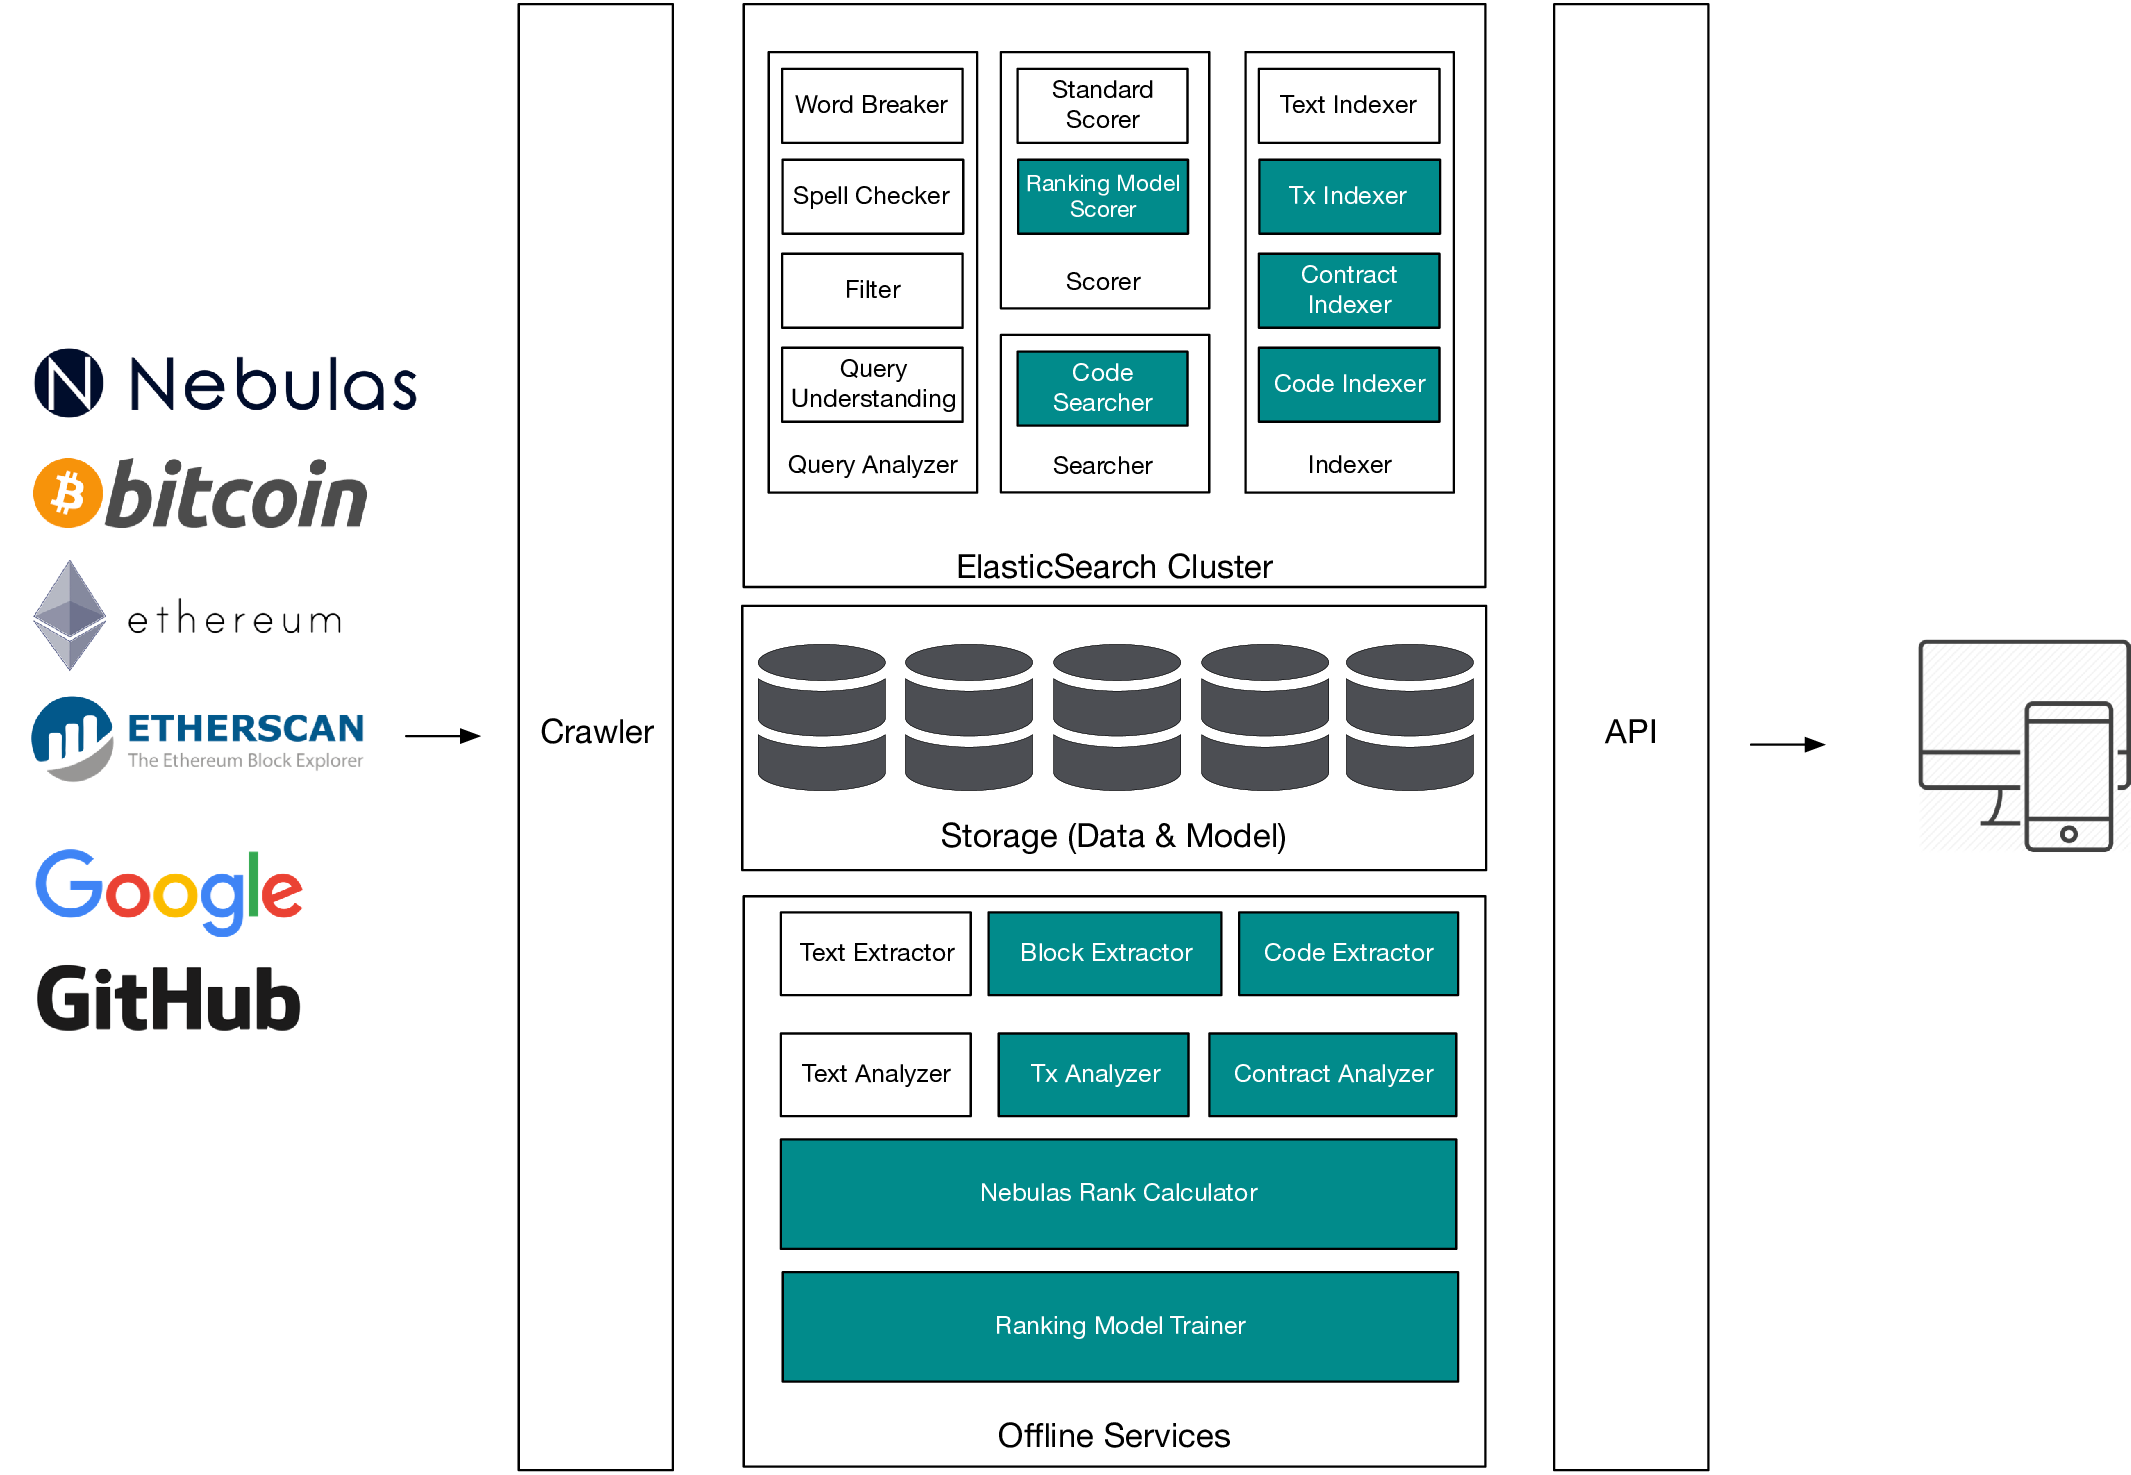
\includegraphics[width=16cm]{./figs/search-arch-new}
\caption{Arquitectura del servicio de búsqueda}
\label{fig:search-arch}
\end{figure}

\begin{itemize}
	\item \textbf{Crawler} los orígenes de los datos del \textit{crawler} del motor de búsqueda blockchain se clasifican en dos tipos: a) búsqueda de información sobre los bloques y el código de los contratos inteligentes en los blockchains; b) búsqueda de información sobre contratos inteligentes desde URL públicas incluyendo introducciones, comentarios de los usuarios acerca de las Dapps, y noticias relacionadas.

	\item \textbf{Extractor} consiste del Extractor de Texto, del Extractor de Bloques y del Extractor de Código, los cuales proveen servicios de extracción de textos, bloques y código de contratos inteligentes, respectivamente.

	\item \textbf{Analyzer} consiste del Analizador de Textos, del Analizador de Transacciones y del Analizador de Contratos, que brindan información sobre textos, información de transacciones en bloques, y análisis de contratos inteligentes, respectivamente. Este último permite descompilar contratos, extraer sus códigos fuente, realizar análisis semánticos, y más.

	\item \textbf{Nebulas Rank Calculator} se refiere al servicio de cálculo de Nebulas Rank, que se utiliza para computar la valuación NR de cada cuenta, sea de usuarios o contratos.

	\item \textbf{Ranking Model Trainer} hace referencia al servicio de entrenamiento del modelo de valuación. Las reglas de valuación toman en cuenta múltiples factores: coincidencia de campos, relevancia de textos, valuación NR del contrato, cantidad de transacciones efectuadas por el mismo, frecuencia y profundidad, valuación NR del usuario que efectúa una transacción con el contrato, y la seguridad de éste. Basándose en las condiciones de uso reales del usuario, el algoritmo de aprendizaje (el GBDT y las redes neuronales artificiales, o ANN, son opcionales) se utiliza para entrenar el modelo de valuación y puntuación, que además están en constante mejora de acuerdo al \textit{feedback} del usuario. El modelo entrenado se utiliza luego para el \textit{Scorer} del servicio de búsquedas.

	\item \textbf{Query Analyzer} se refiere al servicio de análisis de palabras clave, que incluye el sistema multilingüe \textit{Word Breaker} y el corrector ortográfico (\textit{Spell Checker}).

	\item \textbf{Indexer} se encarga de crear índices apropiados para el Analyzer y da soporte a índices completos e incrementales.

	\item \textbf{Scorer} se clasifica en dos niveles:
	\begin{itemize}
		\item \textbf{Nivel 1} \textbf{Standard Scorer} recupera los conjuntos de resultados del candidato de ElasticSearch, lo cual se hace para recuperar tantos resultados de candidatos como sea posible a través de la clasificación eficiente y efectiva en el cluster de ElasticSearch. Este nivel puede recuperar varios miles de resultados.
		\item \textbf{Nivel 2} \textbf{Ranking Model Scorer} utiliza el modelo de valuación \textit{offline} para calcular y reorganizar la valuación de cada candidato del conjunto de resultados del \textit{nivel 1}. En este nivel, los resultados calculados tienen una precisión abrumadora y pueden ser utilizados directamente por los usuarios.
	\end{itemize}
	\item \textbf{Searcher} es el responsable de comunicarse con el cluster ElasticSearch y empacar y devolver el resultado de la búsqueda al \textit{frontend}.

	\item \textbf{API} le proporciona a las aplicaciones externas servicios de búsqueda completos de API.

	\item \textbf{ElasticSearch Cluster} Se refiere al cluster de servidores. El equipo de desarrollo de Nebulas planea utilizar el motor de búsqueda de código abierto ElasticSearch para dar soporte a la indización de texto completo.

\end{itemize}

\subsection{\textit{Nebulas Trends}}

Este sistema genera, en combinación con Nebulas Rank, la lista de tendencias para brindar valores visuales multidimensionales de usuario en los blockchains.

\begin{itemize}
\item \textbf{Lista Nebulas Rank para direcciones de usuarios.} Muestra la lista NR diaria y las listas NR de cambios rápidos en valuaciones ascendentes y descendentes. Además, con esta lista es posible visualizar la tendencia en la variación de la valuación de cada cuenta y la tendencia en los cambios de salud de la red completa.

\item \textbf{Lista Nebulas Rank para cuentas de contratos inteligentes.} Basándose en los valores NR de las cuentas de usuarios, se calcula la lista NR de las cuentas de los contratos inteligentes, la lista de cambios rápidos en valuaciones ascendentes y descendentes, la tendencia en la variación de cada contrato y el gráfico de tendencias para la cantidad y la frecuencia de uso de los contratos inteligentes en toda la red. Además, se añadirán las listas de contratos de tokens y la lista de estimación de contratos de mercado para mostrar una dimensión más amplia de la información.

\item \textbf{Lista de desarrolladores de contratos inteligentes.} De acuerdo a lo descripta en el punto anterior, la lista de desarrolladores de contratos inteligentes enumera las contribuciones de éstos y los casos de rápido ascenso en el \textit{ranking} con el fin de mostrar tanto las {\dapp}s sobresalientes como sus desarrolladores.

\end{itemize}

\subsection{Consulta de palabras clave}

Mediante una palabra clave o una descripción textual —tal como su título, su función o su autor— los usuarios podrán encontrar, entre cualquier cantidad de contratos inteligentes, aquellos que coinciden con esos criterios. En este momento se encuentran disponibles varios algoritmos sofisticados y maduros para su búsqueda mediante texto. Al utilizar procesamiento de lenguaje natural y tecnologías de índice inverso, es posible ordenar y recuperar de forma eficiente la información almacenada en bases de datos cargadas masivamente de contratos inteligentes. Para ello, se hace uso de la siguiente tecnología:

\begin{enumerate}
	\item Rastreador distribuido orientado a tópicos
	\item Segmentación de palabras multilingüe: la segmentación de palabras es una tarea relativamente simple para los lenguajes occidentales; para las palabras chinas, en cambio, se han puesto a disposición los siguientes algoritmos: coincidencia máxima positiva, coincidencia mínima positiva, segmentación por ruta más corta y segmentación estadística.
	\item Corrección de términos de búsqueda y comprensión semántica
	\item Índice inverso y arquitectura de búsqueda distribuida
	\item Algoritmo de valuación para ordenar los resultados de la búsqueda

\end{enumerate}

Entre esas tecnologías, el algoritmo de valuación trabajará en forma combinada con Nebulas Rank. Específicamente, para crear el grafo de transacciones del blockchain utilizamos las transferencias entre usuarios en el mundo blockchain en forma similar a las relaciones de referencias entre los sitios web de internet. Luego, calculamos la valuación NR de las cuentas que no son de contratos inteligentes por medio del uso de la tecnología NR descripta en la sección \refsec{subsec:leaderrank}, calculamos las valuaciones de los contratos por medio del algoritmo descripto en la sección \refsec{dip:arith}, y finalmente utilizamos los resultados para ordenar los resultados de la búsqueda.

\subsection{Búsqueda de resultados similares para contratos inteligentes}

Es de utilidad para los desarrolladores y algunos usuarios la función de búsqueda de contratos inteligentes con funciones similares de acuerdo al fragmento de un código de contrato dado. Al ser diferente de la búsqueda regular de palabras clave, la búsqueda de código similar tiene sus particularidades. Para implementar una función de búsqueda tal, necesitamos hacer uso de un determinado algoritmo capaz de mensurar la similitud del código en porcentajes.

En el mundo académico actual, los algoritmos de similitud de código se clasifican principalmente en distancia de edición de cadenas, similitud de secuencia de tokens, similitud de árboles de sintaxis abstracta y similitud de grafos de dependencias de programas. Estos algoritmos describen la similitud en términos del texto del código, la estructura y la sintaxis, desde diferentes dimensiones. Al combinar esos cuatro algoritmos, planteamos doce características de similitud en el código de los contratos de Nebulas, entre ellas \textit{Skeleton Tree}, signatura y llamadas a librerías. Para más detalles, consúltese el apéndice \ref{appendix:sim_code}.

De forma similar a las búsquedas basadas en palabras clave, los resultados de búsqueda de contratos inteligentes utilizan el mismo algoritmo de valuación de contratos para ordenar los resultados finales.